\hypertarget{fence-unit-test}{%
\section{Testes unitários com FUnit}\label{fence-unit-test}}

O \emph{framework} \emph{Fence Unit Test}, ou \emph{FUnit}, foi implementado para auxiliar os desenvolvedores de sistemas \emph{Fence} na escrita de testes unitários. Conforme mostrado de forma simplificada pela figura \ref{fig:funit-esq}, definido o método que deseja ser testado como entrada, o desenvolvedor escreve o teste utilizando as ferramentas disponibilizadas pelo \emph{FUnit}, para no final ser fornecido um relatório com o resultado.

\begin{figure}[H]
    \centering
    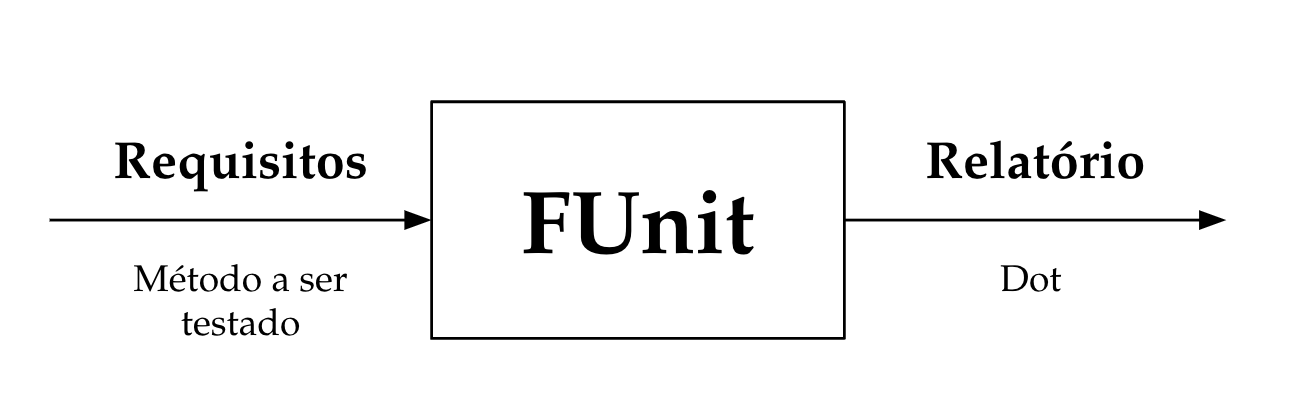
\includegraphics[width=14cm]{source/4-solucao/images/funit-esq.png}
    \caption{Simplificação do \emph{FUnit}. Métodos são usados como entrada e um relatório é gerado no final.}
    \label{fig:funit-esq}
\end{figure}

Esta seção discute o \emph{framework} desenvolvido, explicando primeiramente o \emph{phpunit} e a possibilidade de aprimorar a ferramenta para as necessidades dos desenvolvedores do grupo. É discutido também a implementação do \emph{framework}, com detalhamento de casos de uso e funcionalidades mais avançadas que foram desenvolvidas.

\hypertarget{framework-phpunit}{%
\subsubsection{\texorpdfstring{\emph{Framework phpunit}}{Framework phpunit}}\label{framework-phpunit}}

Para atender o objetivo de pequenas entregas, proposto pela metodologia ágil, é fundamental garantir a qualidade do código. Os testes unitários são essenciais para contribuir para esta garantia, dando início a uma pesquisa por soluções disponíveis para \emph{php}, a linguagem principal do \emph{Fence}. Entre as opções, o \emph{phpunit} é o \emph{framework} dominante na comunidade, sendo a opção escolhida para este projeto.

Estendendo a classe base do \emph{phpunit} por meio do princípio da herança, se torna possível realizar o teste de um método de uma classe, ou da própria classe inteira. Para o caso de um método, por exemplo, é necessário desenvolver um método testador que contenha a execução do método original a ser testado e as nomeadas \emph{condições de controle}, que são os valores de entrada e esperados. O retorno do método original é então comparado com o valor esperado, informando se o teste obteve alguma falha. Na ausência de falhas, o teste é classificado como aprovado. Na figura \ref{fig:phpunit-framework} pode ser visto um exemplo simples deste processo.

\begin{figure}[H]
    \centering
    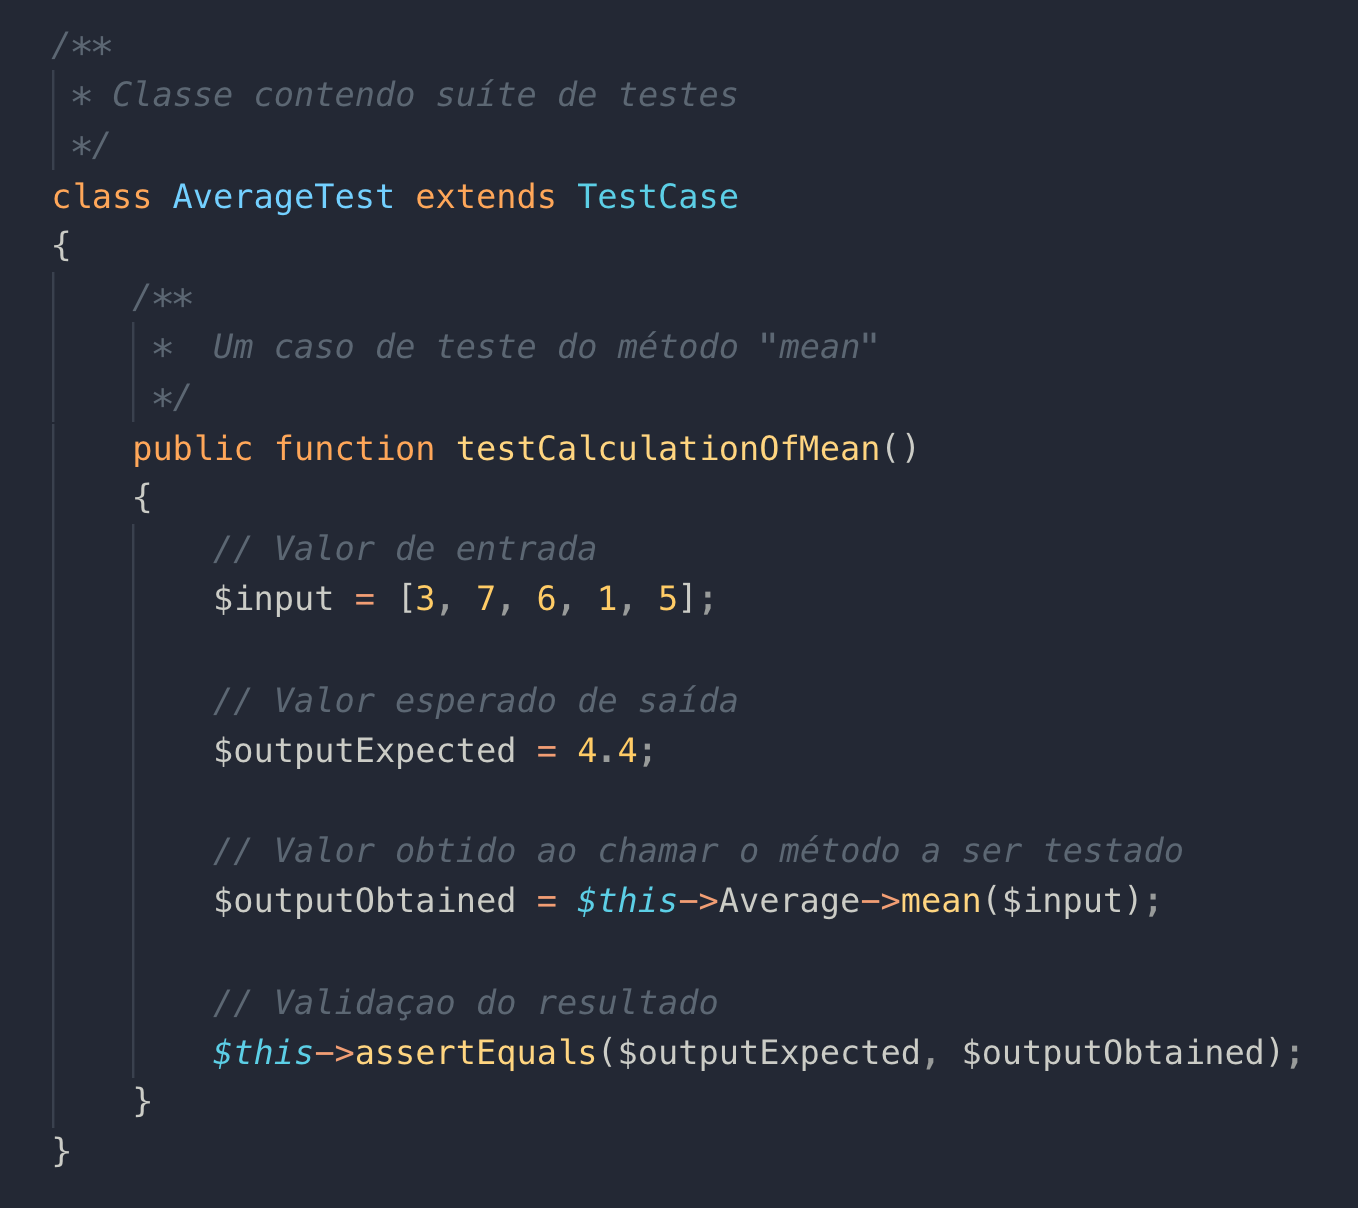
\includegraphics[width=13cm]{source/4-solucao/images/phpunit-framework.png}
    \caption{Exemplo simplificado de um teste unitário.}
    \label{fig:phpunit-framework}
\end{figure}

No contexto da teoria de testes, cada método testador é definido como \emph{~test case}, ou caso de teste, enquanto o agrupamento de \emph{test cases} por sua vez é chamado de \emph{test suite}, ou suíte de testes. É de costume um ou mais \emph{test cases} validarem cada método de uma classe, e o conjunto de todos os \emph{test cases} que percorrem a classe ser um \emph{test suite}. Quando executado, o \emph{phpunit} percorre os \emph{test suites} desejados e exibe os resultados de todos os \emph{test cases} presentes.

\hypertarget{busca-por-padronizacao-e-concisao}{%
\subsubsection{Busca por padronização e concisão}\label{busca-por-padronizacao-e-concisao}}

No passado, alguns testes de unidade foram experimentalmente desenvolvidos pelo grupo com o propósito de incorporar a prática no futuro junto ao processo de desenvolvimento. Entretanto com o crescimento do número de testes foi possível identificar pontos a serem aprimorados. Foi analisado que a escrita dos testes poderia ser padronizada e otimizada. Viu-se a oportunidade em adaptar setores do \emph{framework} para o contexto do grupo, podendo tornar mais econômico e mais rápido para o desenvolvedor desenvolver testes rotineiramente.

Notou-se a possibilidade de melhoria na organização nos \emph{test cases} e suas \emph{condições de controle}. No exemplo anterior e como era feito inicialmente pelos desenvolvedores do grupo, estas condições eram definidas juntamente com a lógica do teste, ou seja, no mesmo código, podendo inclusive ocorrer repetições entre testes que possuíssem as mesmas condições. Esta implementação é satisfatória para uma certa ordem de grandeza de testes, porém quando se passa a ter milhares de testes unitários, dificulta-se a manutenção destes testes. O desenvolvedor precisa procurar em que linhas de código a \emph{condição de controle} foi definida, sem indicativos claros de sua localização e sem uma padronização de como esta condição foi estabelecida. Idealmente as \emph{condições de controle} deveriam estar desatreladas da lógica do teste, sem repetições e seguindo um padrão claro, que facilite a compreensão e manutenção.

Para facilitar o desenvolvimento dos testes pelos programadores, percebeu-se também a possibilidade de simplificar procedimentos mais complexos. Isso ocorre principalmente na simulação de objetos, conhecidos como \emph{mocks}. Para testes unitários simples, em que não ocorre chamadas a outros métodos da classe, \emph{mocks} são desnecessários. Contudo, na maioria dos casos, um método a ser testado possuirá chamadas a outros métodos da mesma classe, e levando em consideração os princípios da prática de teste unitário, o comportamento destas chamadas precisa ser controlado. Um teste unitário não pode possuir dependências externas, como a outros métodos que podem ter comportamentos imprevisíveis, pois isso prejudicaria a natureza modular do teste. Portanto conclui-se que \emph{mocks} são necessários, e apesar do \emph{phpunit} possuir funcionalidades nativas para criá-los, grande parte dos comandos podem ser simplificados, reduzindo a prolixidade da escrita.

Levando em consideração principalmente estes dois motivos, foi proposta a implementação de uma camada acima do \emph{framework} \emph{phpunit}, que passaria a ser a nova ferramenta para desenvolvimento de \emph{test suites} do grupo. Esta camada tem como objetivo principal implementar um padrão conciso na escrita de testes unitários, guiando o desenvolvedor durante a escrita do teste. Pelo fato de ser uma abstração motivada para testar código relacionado com o \emph{framework} \emph{Fence}, esta ferramenta foi nomeada \emph{Fence Unit Test}.

\hypertarget{desenvolvimento-do-framework-funit}{%
\subsubsection{\texorpdfstring{Desenvolvimento do \emph{framework} \emph{FUnit}}{Desenvolvimento do framework FUnit}}\label{desenvolvimento-do-framework-funit}}

\emph{FUnit} foi inspirado nos princípios seguidos pelo próprio \emph{Fence}. Através do \emph{Fence}, os parâmetros sujeitos a mudanças constantes são abstraídos em arquivos de configuração, de modo que até mesmo o próprio usuário possa ser capaz de alterá-los em certos casos. A premissa é semelhante ao \emph{FUnit}, na medida que as \emph{condições de controle} são exteriorizadas em um arquivo \emph{JSON}. Dessa forma, torna-se possível para o desenvolvedor alterar o valor de entrada ou da saída esperada sem a necessidade de alterar o código do próprio teste.

O Fence Unit Test constitui um \emph{namespace}, \emph{/Fence/UnitTest}, o qual possui uma classe principal, a \emph{TestCase}, responsável pela maior parte da lógica do \emph{framework}, e a classe secundária, \emph{Assert}, encarregado de asserções. Juntamente com a orientação a objetos, estas classes foram escritas baseando-se parcialmente no paradigma funcional, evitando mudanças de estado e dados mutáveis. Optou-se pela estruturação em pequenos métodos, dependentes apenas de seus argumentos, e gerar novas variáveis ao invés de reutilizá-las.

Aplicou-se também dois princípios da filosofia \emph{SOLID} para o \emph{FUnit}. Primeiramente foi utilizado o princípio da inversão de dependências, no qual as classes desenvolvidas possuem dependência apenas de outras classes abstratas, e o princípio da responsabilidade única, de modo que os métodos foram planejados para cumprirem unicamente uma tarefa.

Com o objetivo de dar mais opções na escrita de arquivos de configuração, foi implementado uma classe auxiliar de processamento de arquivos \emph{JSON} chamada \emph{JProcessor}. Esta classe interpreta o arquivo de configuração realizando mudanças de acordo com certas regras. Ações como capacitação de comentários, substituição de variáveis globais, concatenação de arquivos de configuração e execução de funções \emph{callback} são possíveis por meio da classe \emph{JProcessor}, se tornando um utilitário que é utilizado pelos desenvolvedores para além do desenvolvimento de testes.

\hypertarget{como-desenvolver-um-teste-unitario}{%
\subsubsection{Como desenvolver um teste unitário}\label{como-desenvolver-um-teste-unitario}}

Observando o funcionamento interno da \emph{FUnit} é possível identificar as etapas bem definidas ao longo do processo de desenvolvimento de testes, como presente na figura \ref{fig:funit-phpunit}. Definido o método a ser testado, considerado como requisito, é possível dar início ao processo de desenvolvimento do teste. Em resumo, \emph{condições de controle} são declaradas em arquivos de configuração e interpretados por uma classe auxiliar que as disponibiliza para a escrita da lógica do teste. Os testes são então executados e validados, gerando um relatório final com os resultados.

\begin{figure}[H]
    \centering
    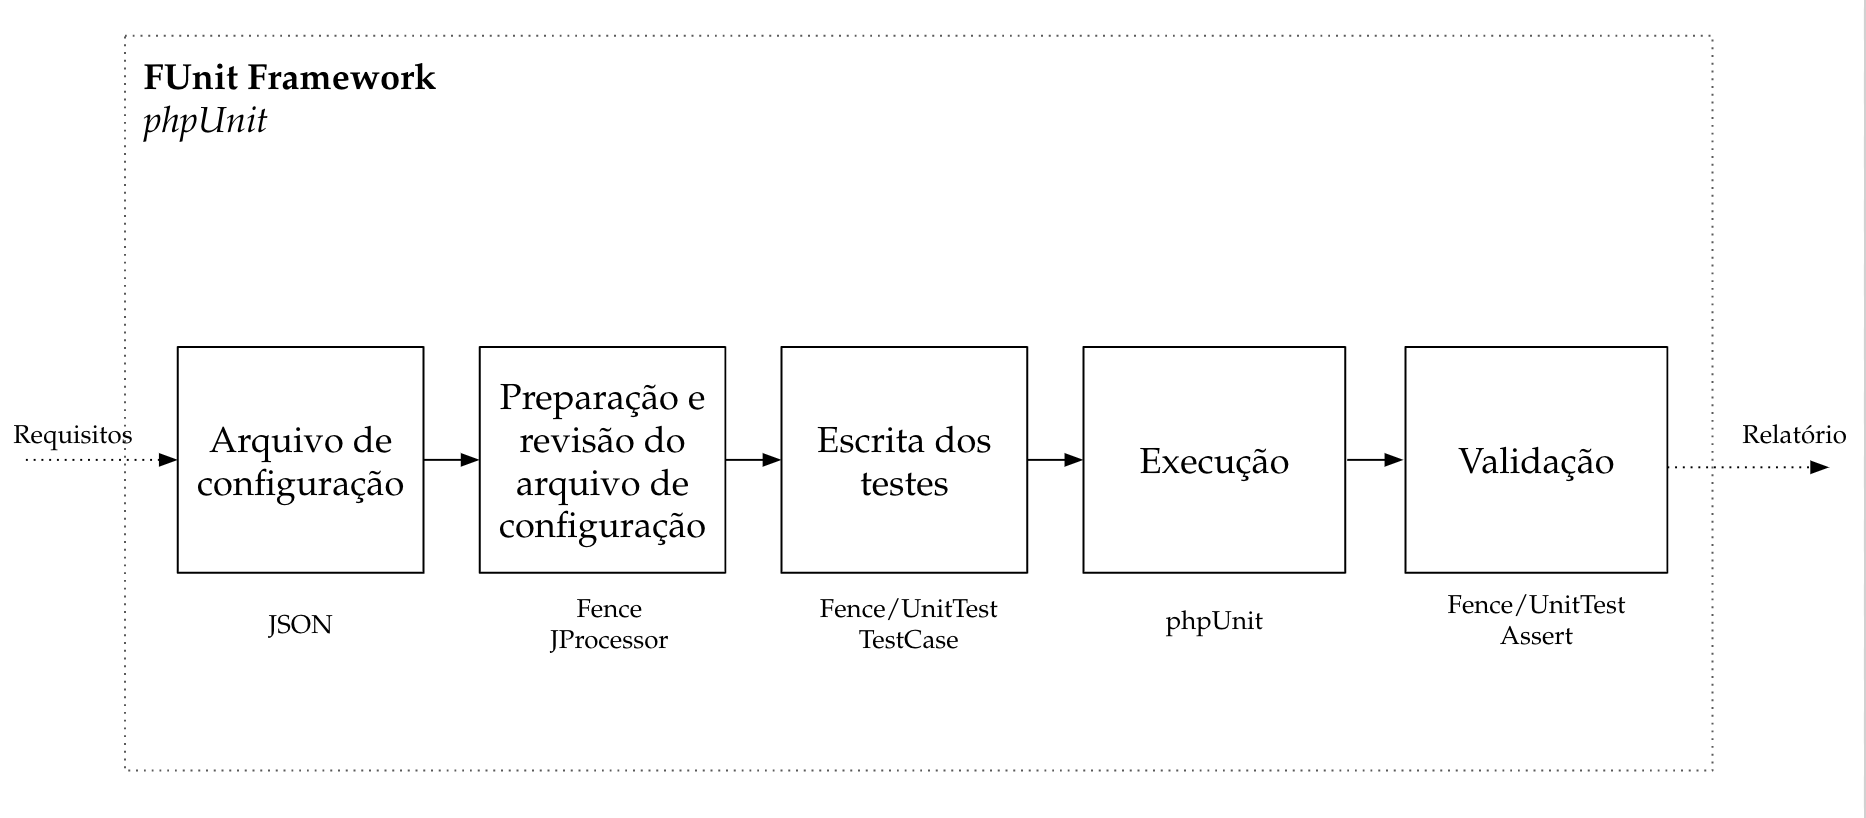
\includegraphics[width=14cm]{source/4-solucao/images/funit-phpunit.png}
    \caption{Funcionamento interno do \emph{FUnit}.}
    \label{fig:funit-phpunit}
\end{figure}

A figura \ref{fig:metodo-testado} exibe um exemplo de método a ser testado. Este método se trata apenas de um atribuidor de propriedades que armazena o nome de um arquivo na instância da classe. Chamado \emph{setFilename} este método faz parte da classe \emph{FileManager} responsável por gerenciar arquivos. Ele possui dois comportamentos distintos, um para o caso de sucesso, e outro para o caso de falha. Na eventualidade do argumento recebido não ser um arquivo, uma exceção deve ser executada, notificando o desenvolvedor do erro. Caso contrário, o nome do arquivo é armazenado como uma propriedade da classe. Portanto, pode-se concluir que dois testes unitários são necessários para esse método, validando cada comportamento possível.

\begin{figure}[H]
    \centering
    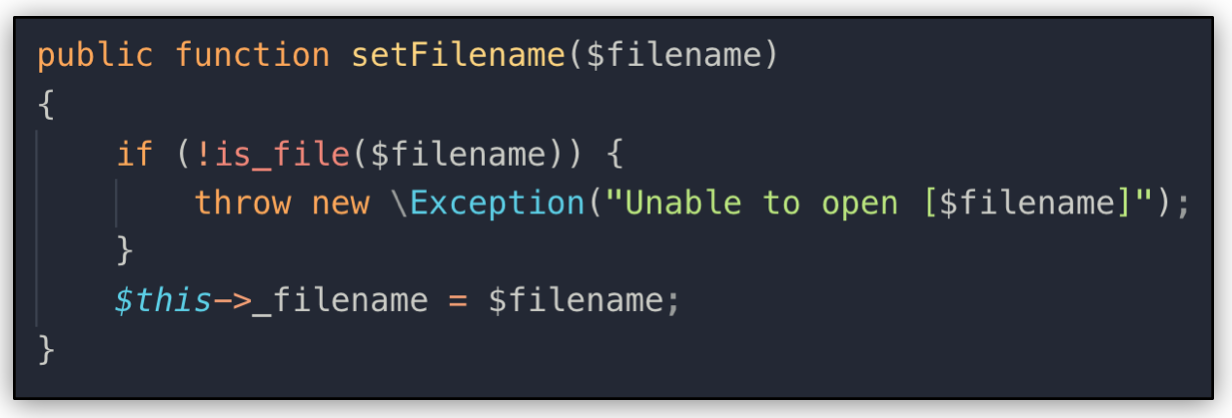
\includegraphics[width=13cm]{source/4-solucao/images/metodo-testado.png}
    \caption{Método a ser testado pelo teste unitário.}
    \label{fig:metodo-testado}
\end{figure}

É necessário antes de tudo a preparação de um arquivo \emph{JSON} de configuração que proporcione as \emph{condições de controle} do teste, como presente na figura \ref{fig:condicoes-de-controle}. Este arquivo inicialmente possui a propriedade \emph{testSetFilename}, que contém as condições necessárias para o desenvolvimento do \emph{test case} de \emph{setFilename}. Dentro desta propriedade, pode-se ver a subpropriedade \emph{class} apontando para o \emph{namespace} da classe \emph{FileManager}, com a condição de construtor desabilitada, denominado \emph{constructor}. Isso significa que um \emph{mock} da \emph{FileManager} será gerado sem a exigência de executar o construtor da classe. Em seguida pode-se ver a subpropriedade \emph{input} que por sua vez possui dois atributos. Estes atributos declaram a entrada para cada teste unitário deste método, sendo um para o comportamento em que se armazena o valor e o outro para quando ocorre a exceção. No fim do arquivo tem-se a propriedade \emph{output}, que contém o valor a ser armazenado pelo método testado, no caso sendo o mesmo valor de \emph{input}.

\begin{figure}[H]
    \centering
    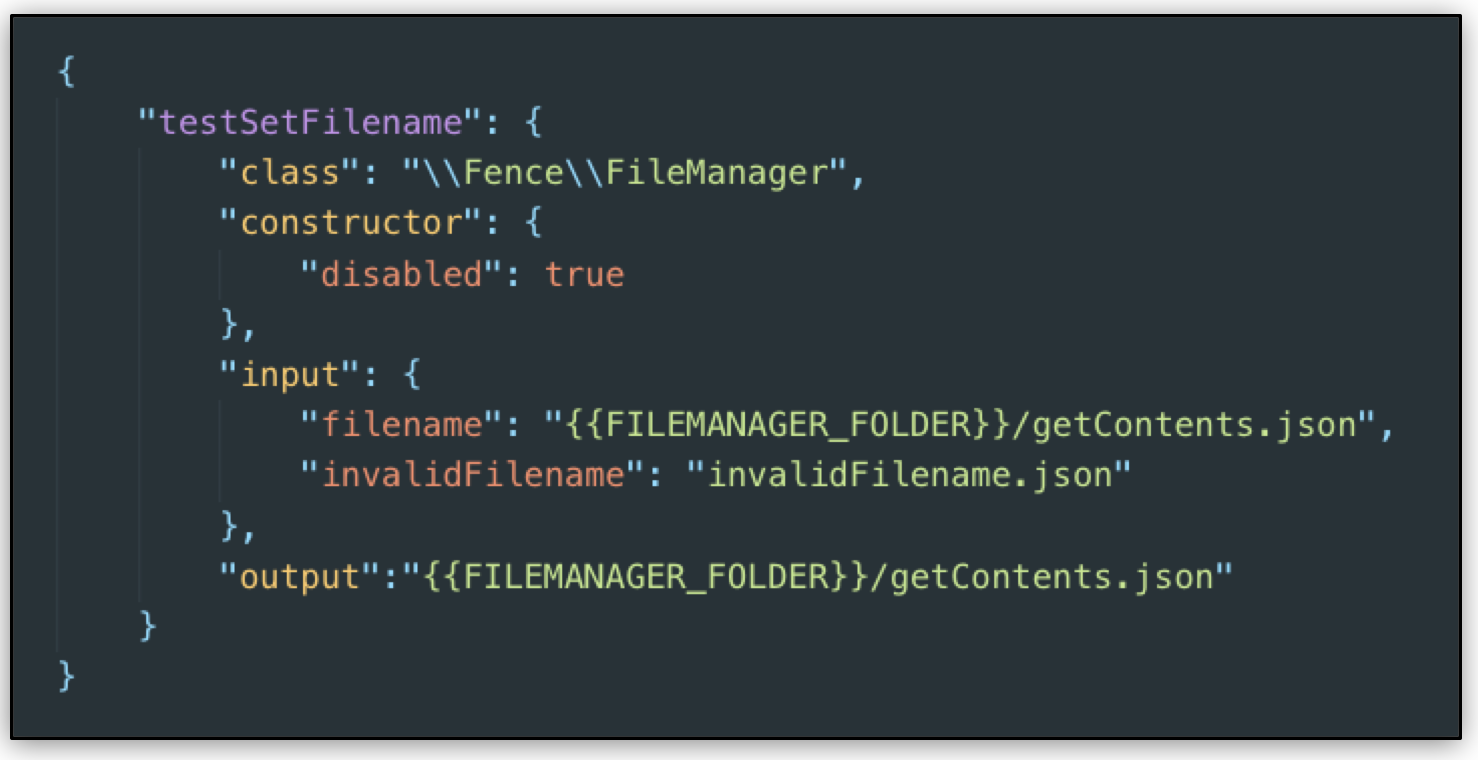
\includegraphics[width=13cm]{source/4-solucao/images/condicoes-de-controle.png}
    \caption{Arquivo de configuração com as condições de controle para teste.}
    \label{fig:condicoes-de-controle}
\end{figure}

Finalizado o arquivo, resta escrever a classe de teste \emph{FileManagerTest}, que estende a classe \emph{TestCase} do \emph{FUnit}. A \emph{TestCase} irá automaticamente invocar a classe \emph{JProcessor} para realizar um pré-processamento do arquivo de configuração. A \emph{JProcessor} irá realizar as traduções necessárias e decodificar o arquivo da estrutura \emph{JSON} para a estrutura de dados compatível com a linguagem \emph{php}.

Dentro da classe \emph{FileManagerTest}, ilustrada na figura \ref{fig:logica-do-teste}, é desenvolvido um dos métodos de teste, o \emph{testSetFilename}, que valida o valor armazenado. Este método por sua vez executa o principal método da \emph{TestCase}, chamado \emph{setTestCaseWithMock}, que é o responsável por tornar disponíveis as informações do arquivo de configuração. A partir disso se obtém o valor do argumento a partir do \emph{input} que será usado pelo método \emph{setFilename}. O retorno do método é por fim comparado com o valor esperado, por meio do método \emph{assertSame} que é disponibilizado por intermédio da classe \emph{Assert}. Quando o teste é executado pela linha de comando \emph{phpunit}, é acusado o erro caso haja divergência entre os valores.

\begin{figure}[H]
    \centering
    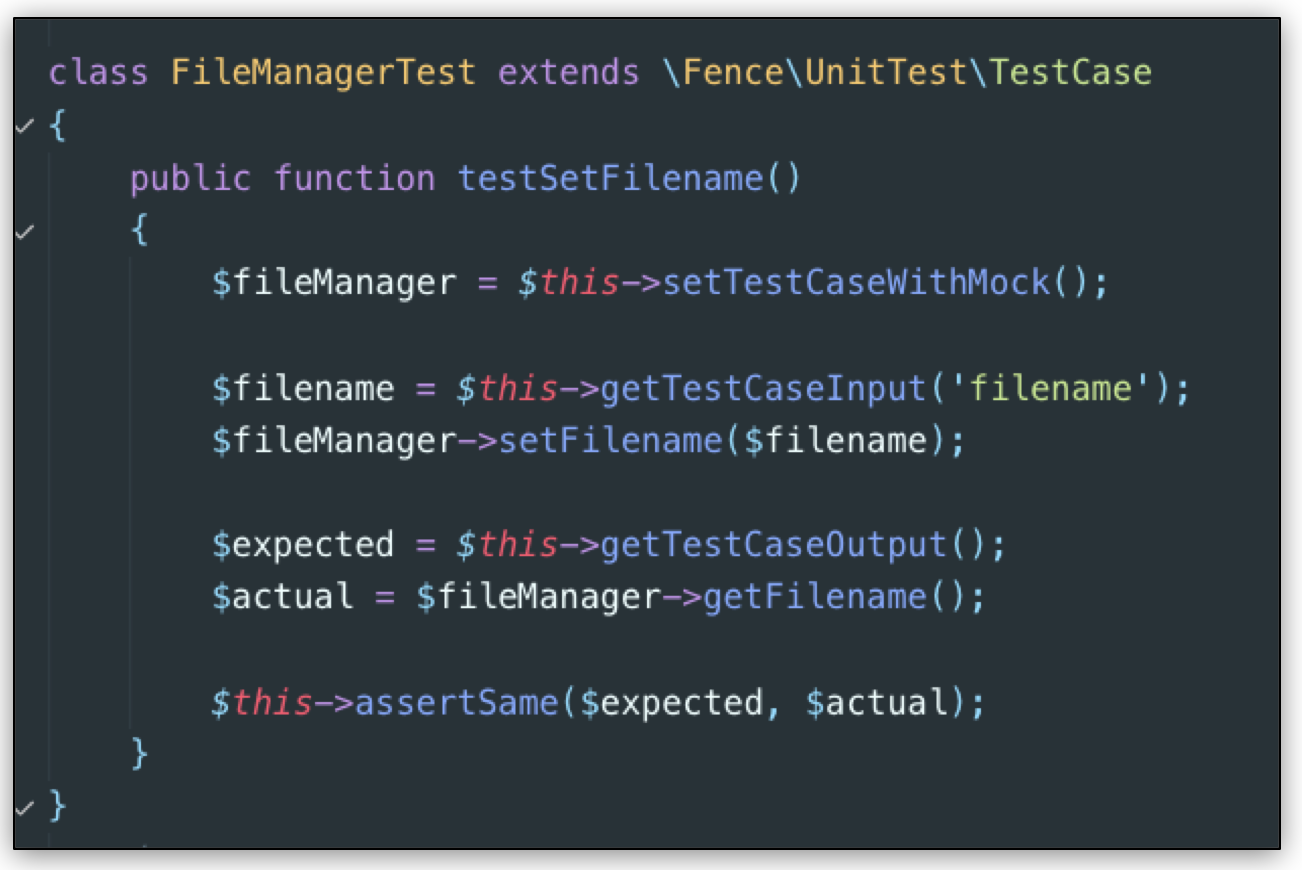
\includegraphics[width=13cm]{source/4-solucao/images/logica-do-teste.png}
    \caption{Lógica do teste do método.}
    \label{fig:logica-do-teste}
\end{figure}

Utilizando a mesma classe e o mesmo arquivo de configuração, o programador pode repetir o processo e desenvolver mais testes até que seja atingida a cobertura de código desejada para a classe a ser testada.

\hypertarget{funcionalidades-adicionais}{%
\subsubsection{Funcionalidades adicionais}\label{funcionalidades-adicionais}}

Com o início do uso do \emph{FUnit}, observou-se a necessidade de funcionalidades adicionais, que estão exemplificadas na figura \ref{fig:funcionalidades-add}. Primeiramente foi desenvolvido o conceito de \emph{~Mocked Methods}, no qual é possível controlar a resposta de um método pertencente a um \emph{mock}. Isso se torna essencial para testar métodos que fazem chamadas a outros métodos de mesma classe.

Como visto no exemplo anterior, o \emph{FUnit} permite também ter múltiplas condições de entrada ou de saída no arquivo de configuração. Isto se torna extremamente útil quando é necessário verificar diferentes comportamentos para um mesmo método a ser testado.

Tornou-se possível também a possibilidade de passar argumentos para o construtor do \emph{mock} quando habilitado. Na maior parte dos casos, não é necessário executar o construtor, já que dado o princípio do teste unitário ser isolado, o próprio independe da execução do construtor. Entretanto, para testar múltiplos módulos, como é o caso dos testes de integração, esta ferramenta pode ser útil.

Apesar do \emph{phpunit} possuir uma biblioteca nativa com asserções disponíveis para diversas estruturas de dados, se tornou essencial a possibilidade de gerar asserções adicionais, personalizadas para os \emph{test cases} do projeto. Para esse intuito a classe auxiliar \emph{Assert} foi desenvolvida, a qual estende as asserções nativas do \emph{phpunit} e permite a escrita de novas asserções conforme a necessidade.

Por fim tem-se no \emph{FUnit} a possibilidade de compartilhar propriedades em comum dentro do próprio arquivo de configuração. Foram desenvolvidos métodos híbridos no \emph{FUnit} que, na ausência de uma \emph{condição de controle} dentro da propriedade do \emph{test case}, procura automaticamente na raiz do arquivo. Esta funcionalidade foi gerada principalmente para o compartilhamento de configurações de \emph{mock}, já que geralmente os \emph{test cases} de uma \emph{test suite} utilizam a mesma classe como referência de \emph{mock}.

\begin{figure}[H]
    \centering
    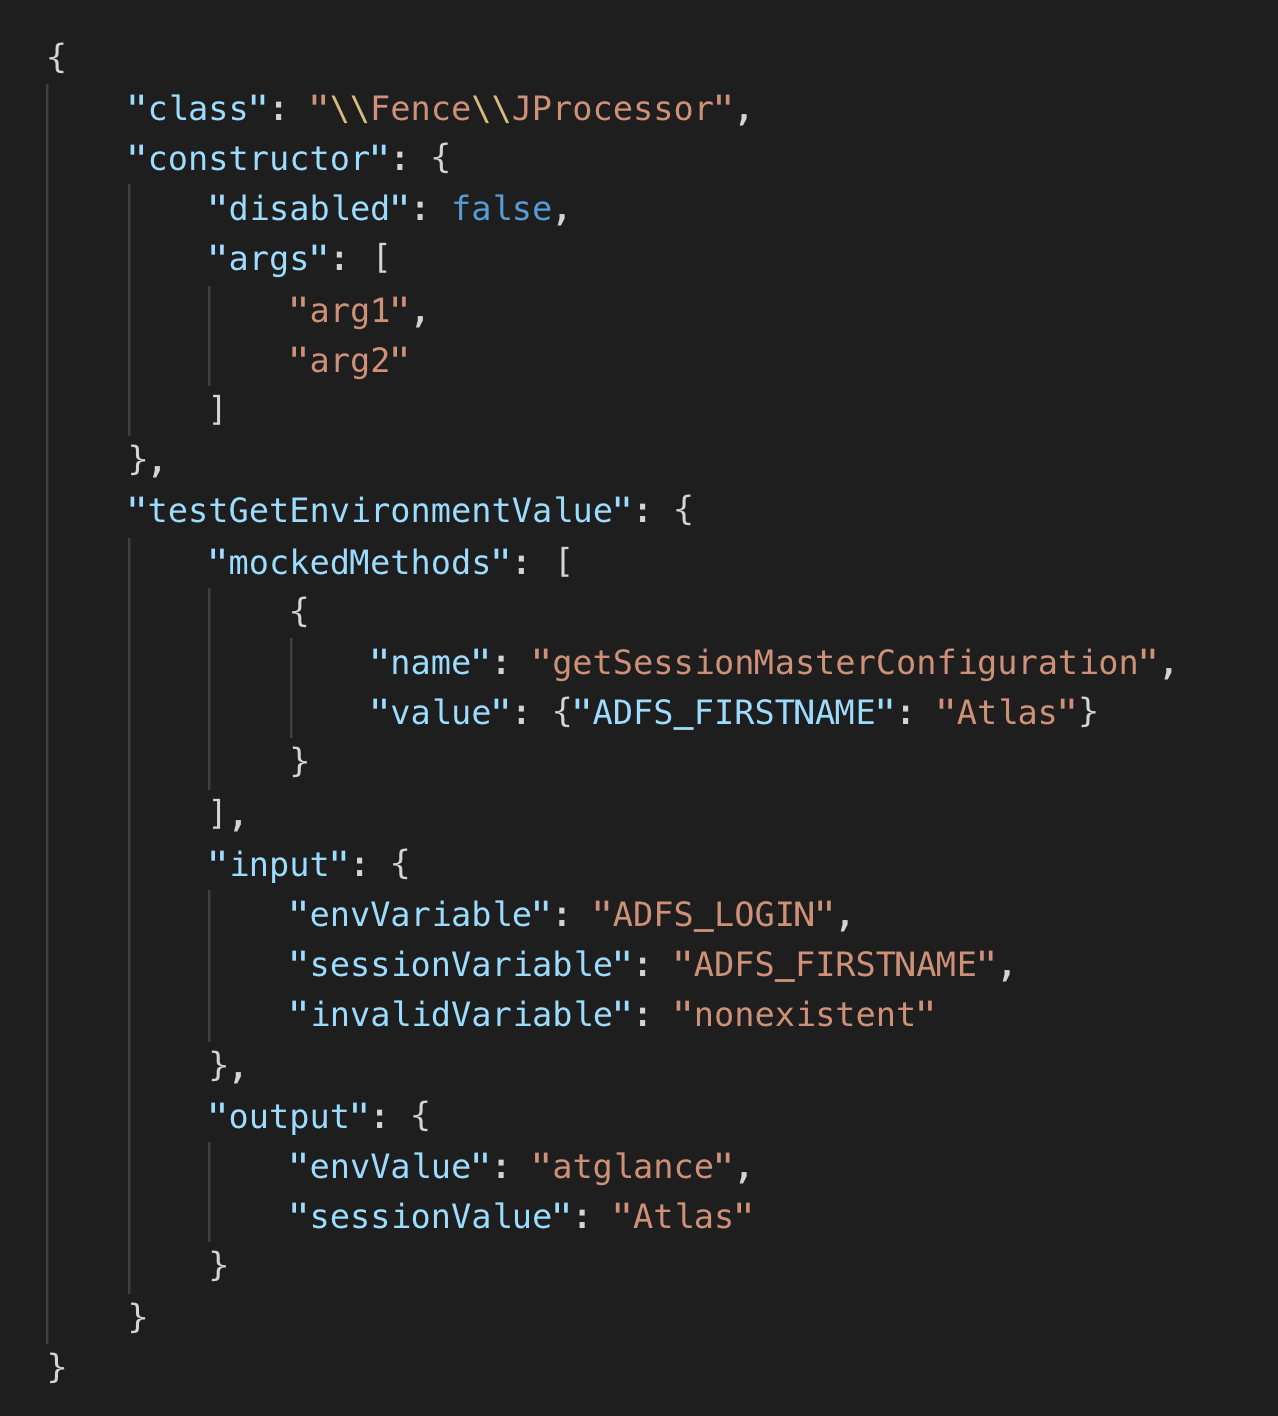
\includegraphics[width=13cm]{source/4-solucao/images/funcionalidades-add.png}
    \caption{Exemplo mais sofisticado de um arquivo de configuração provido à \emph{FUnit}.}
    \label{fig:funcionalidades-add}
\end{figure}

Discutida as principais características do \emph{framework} \emph{FUnit}, a próxima seção discute o framework \emph{Fate}, voltado para testes \emph{e2e}.
